\documentclass[a4paper,11pt]{style-esi/td}

\usepackage{style-esi/licence}
\usepackage{style-esi/exercice}
\usepackage{style-esi/exemple}
\usepackage{style-esi/question}
\usepackage{style-esi/tutoriel}
\usepackage{style-esi/listing}
\usepackage{style-esi/images}
\usepackage{style-dev1/dev1}
\usepackage{longtable} % Pour des tables sur plusieurs pages

\begin{document}

\seance{3}{Java sur linux}
\entete
\titre
\ccbysa{esi-dev1-list@he2b.be}
\lastedit

\bigskip
\begin{abstract}
    Lorsqu'on programme en \name{Java} sur \name{Linux},
    on peut, comme sur \name{Windows},
    utiliser un environnement de développement comme \name{Netbeans}.
    Mais on peut aussi tout faire en mode console, 
    c'est ce que nous allons voir ici.
    Nous en profiterons pour apprendre de nouvelles notions liées à Linux.
\end{abstract}

\bigskip
\tableofcontents

\vfill
\begin{infobox}
    Dans votre répertoire \samp{home/dev1}, 
    créez un répertoire \samp{td3}. 
    Ce répertoire contiendra tous les fichiers que vous allez créer aujourd'hui. 
\end{infobox}

\newpage

%============================================================
\section{Quelques notions supplémentaires de Linux}
%============================================================

	Avant d'attaquer le c\oe{}ur du TD, 
	à savoir le compilation et l'exécution de programmes Java,
	voyons quelques éléments e Linux qui vous seront utiles.

	%============================================================
	\subsection{La ligne de commande}
	%============================================================
              
		Commençons par quelques astuces 
		pour vous faciliter la vie lorsque vous entrez des commandes.
		
		\subsubsection*{La complétion de commandes}
		%======================================

			Parfois, vous devez entrer une commande assez longue 
			parce que les noms de fichiers sont longs et/ou nombreux.
			Linux offre plusieurs facilités pour simplifier l'entrée de longues commandes.  

			Lorsque vous appuyez sur la touche \samp{TAB}, 
			le shell tente de compléter le début de commande 
			que vous avez déjà tapé. 
			Si plusieurs possibilités existent, 
			elles sont affichées si vous appuyez 2x sur \samp{TAB}.  

			\begin{Tutoriel}{La complétion de la commande} 
				Supposons que vous ne vous rappeliez plus très bien 
				de la commande qui permet de modifier le mot de passe.
				Vous vous rappelez juste qu'elle commence par \kbd{pas}.  
				\begin{steps}
				\item 
					Tapez \kbd{pas} puis appuyez 2x sur la touche \samp{TAB}.
				\item 
					Entrez un \kbd{s} puis appuyez à nouveau sur \samp{TAB}.
				\end{steps}
			\end{Tutoriel}		
			
			\medskip
			La touche de tabulation permet également de compléter un nom de fichier.

			\begin{Exercice}{La complétion des noms de fichiers}  
				\vspace{-1em}          
				\begin{enumerate}
				\item 
					Dans votre dossier \samp{td3}, 
					copiez le fichier \par
					\samp{monfichieraunomtellementlongquilmeparaitpeuprobabledeletaper2xsanserreur} 
					qui se trouve dans le dossier \samp{/eCours/java/td/td3}.
				\item 
					Affichez le contenu de ce fichier en évitant de retaper son nom.
				\end{enumerate}
			\end{Exercice}	
			
			% \begin{Exercice}{Joker} 
			% 	Le point 20 du guide visuel parle des jokers; c'est le moment de les utiliser :) 
			% 	\par
			% 	\begin{enumerate}
			% 		\item Copiez dans votre répertoire td3 créé ci-dessus tous les fichiers du répertoire \verb@/eCours/java/td/td3@ dont l'extension est \verb@.java@ 
			% 		(c'est possible sans passer par un \,\verb|cd /eCours/java/td/td3|\,)
					
			%     			\item Copiez dans votre répertoire td3 tous les fichiers du répertoire  \verb@/eCours@\ \verb@/java/td/td3@ dont la deuxième lettre est un '\verb@x@'.
	
			%       		\item  Listez le contenu des répertoires des étudiants (pour rappel, les répertoires des étudiants sont ceux qui se trouvent dans \verb@/home@ et qui 						commencent par un '\verb@g@').
			%  			\item Listez le contenu des répertoires des professeurs (pour rappel, les répertoires des professeurs sont ceux qui se trouvent dans \verb@/home@ et qui 						sont composés de 3 lettres).
			%   		\end{enumerate}
			% \end{Exercice}
								
		\subsubsection*{Revenir à une commande précédente} 
		%==============================================

			Il arrive souvent qu'il faille entrer une commande 
			qu'on a déjà écrite il y a peu 
			(ou en tout cas fort proche de ce qu'on a déjà écrit). 
			C'est là que les flèches viennent à notre secours.  
			
			La flèche vers le haut permet de revenir aux commandes précédentes 
			et de les modifier. À utiliser sans modération\dots  

		\subsubsection*{Historique des commandes} 
		%==============================================
		
			\begin{itemize}
			\item \kbd{history} : 
				affiche la liste des dernières commandes entrées.
				Chaque commande est numérotée.
			\item \kbd{!numéro} : 
				ré-execute la commande de numéro donné.
			\item \kbd{!cmd} : 
				ré-execute la dernière commande qui commençait par \samp{cmd}.
			\end{itemize}

	%============================================================
	\subsection{Les fichiers cachés}
	%============================================================

		\begin{theorie}{Les fichiers cachés}
			Un \textbf{fichier caché}
			est un fichier
			dont le nom commence par \og{}\samp{.}\fg{} (un point).
			\\
			Idem pour un dossier.
		\end{theorie}

		Par défaut, 
		les fichiers cachés ne sont pas montrés par la commande \kbd{ls}.
		Pour les voir, utiliser l'option \texttt{a} : \kbd{ls -a}.
		C'est surtout utilisé pour des fichiers de configuration.

		\begin{Exercice}{Les fichiers cachés de la home}
			Regardez s'il existe des fichiers cachés
			dans votre répertoire personnel.
		\end{Exercice}

%=====================================
\section{L'éditeur nano}
%======================================

	Un éditeur de texte, même simple comme nano,
	peut apporter quelques facilités dans l'écriture de programmes.

	\subsection{Coloration syntaxique}
	%=================================

		La coloration syntaxique signifie 
		utiliser des couleurs pour mettre en évidence certaines parties d'un code :
		mots clés, constantes\dots{}
	
		Pour utiliser cette facilité, 
		il faut configurer \name{nano}. 
		Cette configuration se fait dans le fichier \samp{\textasciitilde{}/.nanorc}.

		\begin{Tutoriel}{Introduire la coloration sytaxique} 
			\vspace{-1em}
			\begin{steps}
			\item 
				Tapez \kbd{nano \textasciitilde/.nanorc} 
				pour éditer le fichier de configuration de \emph{nano}.
			\item 
				Ajoutez-y la ligne : \samp{include "/usr/share/nano/java.nanorc"}
			\item 
				Quittez l'éditeur.
			\item 
				Ouvrez le fichier \samp{Ex.java};
				il devrait être coloré.
			\end{steps}
		\end{Tutoriel}
				
	\subsection{Numérotation des lignes}
	%=================================
				
		Nano peut également indiquer le numéro de la ligne sur laquelle se trouve le curseur, 
		ce qui sera pratique pour corriger vos erreurs. 
		Pour cela, il existe deux méthodes.

		\begin{itemize} 
		\item \textbf{Méthode 1} : 
			Lancer nano avec l'option \samp{-c} : \kbd{nano -c monFichier}.
		\item \textbf{Méthode 2} : 
			Dans l'éditeur, appuyez sur \samp{CTRL-c}.
		\end{itemize}
			
	\subsection{Indentation}
	%=================================
				 
		Pour qu'un programme soit lisible, 
		il doit être \textit{indenté}. 
		Ce qui serait pratique lorsqu'on code ce serait qu'un retour à la ligne 
		positionne automatiquement le curseur de façon à être aligné avec la ligne précédente. 
		Pour que nano fasse ça pour nous, 
		il suffit d'ajouter	ceci à son fichier de configuration : \samp{set autoindent}.
			
	\subsection{Autres configurations} 
	%=================================
		
		Si vous désirez connaitre d'autres possibilités de configuration de nano, 
		vous pouvez lire le manuel : \kbd{man nanorc}.

		Pour une \textit{quick ref} en ligne, consultez (par exemple) : \\
		\url{www.codexpedia.com/text-editor/nano-text-editor-command-cheatsheet/}
		.

%=============================
\section{Compiler et exécuter du Java}
%==============================

    \begin{theorie}{Java sans package}
        Si le programme Java n'utilise pas de package :
        \begin{itemize}
            \item \kbd{javac MaClasse.java} compile le programme Java du fichier donné
            \item \kbd{java MaClasse} : exécute le programme Java se trouvant dans la classe donnée.
        \end{itemize}
    \end{theorie}

	\begin{Tutoriel}{Compiler / exécuter un programme} 
		Commençons par un programme correct et tentons de l'exécuter.  
      
        Le fichier \samp{/eCours/java/td/td3/Ex.java} 
        contient un petit programme Java tout simple qui affiche un message de bienvenue. 
        
		\begin{steps}	
        \item 
            Si ce n'est pas le cas, placez-vous dans le dossier \samp{td3}.
        \item 
            Copiez le fichier indiqué dans cd dossier :
            \kbd{cp /eCours/java/td/td3/Ex.java .}
        \item 
            Lisez-le et voyez si vous devinez ce qu'il fait : \kbd{cat Ex.java}
        \item 
            Compilez-le : \kbd{java Ex.java}
        \item 
            Que fait cette phase, à quoi sert-elle ?
            Affichez le contenu du dossier pour le vérifier.
		\item Exécutez le programme : \kbd{java Ex}
		\end{steps}			
	\end{Tutoriel}

    Lorsqu'on compile, il faut mettre le \samp{.java} 
    mais lorsqu'on exécute, 
    il ne faut pas mettre le \samp{.class}.

    \begin{alerttbox}{Retenez !} 
        On \textbf{compile un fichier} mais on \textbf{exécute une classe}.
    \end{alerttbox}

	Vous allez à présent écrire votre premier programme de bout en bout sur linux1. 
	
	\begin{Exercice}{Un programme Java}
		Écrivez un programme qui :
		\begin{itemize}
		\item Affiche votre nom ;
		\item Affiche la valeur de $7^2$ ;
		\item Affiche la valeur de $2^7$ ;
		\item Demande une entier à l'utilisateur et affiche s'il est pair. 
		\end{itemize}
	\end{Exercice}

	\begin{alerttbox}{Conseils}
		Procédez par étape et vérifiez correctement votre programme.
		Ce n'est pas parce qu'il compile qu'il est correct.
		Et ce n'est pas parce qu'il affiche quelque chose que c'est la bonne réponse.
	\end{alerttbox}

	\begin{Exercice}{Comprendre les erreurs (I)}
		Supposons que vous faites une erreur dans votre programme.
		Par exemple en écrivant \code{java}{Public} 
		au lieu de \code{java}{public}.

		À quelle étape le problème va-t'il apparaitre ?
		Sous quelle forme ? Testez !
	\end{Exercice}

	\begin{Exercice}{Comprendre les erreurs (II)}
		Supposons que vous demandez un calcul impossible dans votre programme.
		Par exemple \code{java}{1/0}.

		À quelle étape le problème va-t'il apparaitre ?
		Sous quelle forme ? Testez !
	\end{Exercice}

%=================================
\section{Transfert de fichiers}  
%=================================

	Vous n'avez peut-être pas fini. Pour pouvoir continuer à la maison sans tout recommencer, 
    il serait bon de pouvoir récupérer ce que vous avez déjà fait sur linux1.
	Voici une façon de le faire.			
				
	\begin{Tutoriel}{Transférer des fichiers}
	\begin{steps}		
		\item 
			Ouvrez l'explorateur de fichier Windows (par exemple en cliquant sur l'icône "My Computer").
		\item 
			Dans le champ d'adresse, tapez l'adresse \samp{ftp://linux1}.
		\item 
			Une boite de dialogue vous demande votre login et mot de passe (sur \textit{linux1}).
		\item 
			Vous voyez apparaitre votre dossier personnel sur \textit{linux1}. 
		\item 
			Vous pouvez y prendre/déposer des fichiers comme vous le feriez pour un dossier Windows. 
			Vous pouvez par exemple les mettre sur une \textbf{clé USB},
			sur le cloud ou vous les envoyer par mail.
	\end{steps}
	\end{Tutoriel}			

%===================
\section{Conclusion}
%====================

	\subsection{Ce qu'il faut connaitre}
	%===================================

		\begin{theorie}{Notions importantes de ce TD}
			Voici les notions importantes que vous devez avoir assimilées à la fin de ce TD.
			\begin{itemize}
			\item 
				La notion de fichier caché et comment les voir.
			\item 
				Savoir utiliser \samp{nano} pour éditer un petit programme Java.
			\item 
				Savoir compiler et exécuter un programme Java 
				qui n'utilise pas de package.
			\end{itemize}
		\end{theorie}

	\subsection{Pour aller plus loin : l'éditeur \texttt{vi}}
	%==================================

		Si vous avez fini,
		vous serez peut-être curieux d'apprendre à utiliser \texttt{vi}
		plutôt que \texttt{nano}.

		Quels sont les avantages de \texttt{vi} ?
		\begin{itemize}
		\item 
			Certaines manipulations du fichiers sont plus simples : 
			copier, supprimer, déplacer des lignes par exemple.
		\item 
			Il est facile d'indenter proprement un programme Java qui ne l'est pas.
		\end{itemize}

		\texttt{vi} est plus puissant que \texttt{nano}
		mais il est moins intuitif quand on débute.
		Voici les bases à comprendre.

		\subsubsection*{Démarrer}
		%========================

			Pour éditer un fichier texte existant
			ou créer un nouveau fichier, 
			il suffit de taper : \kbd{vi monFichier}.

			Les 3 modes de fonctionnement sous vi(m) :
			\begin{center}
			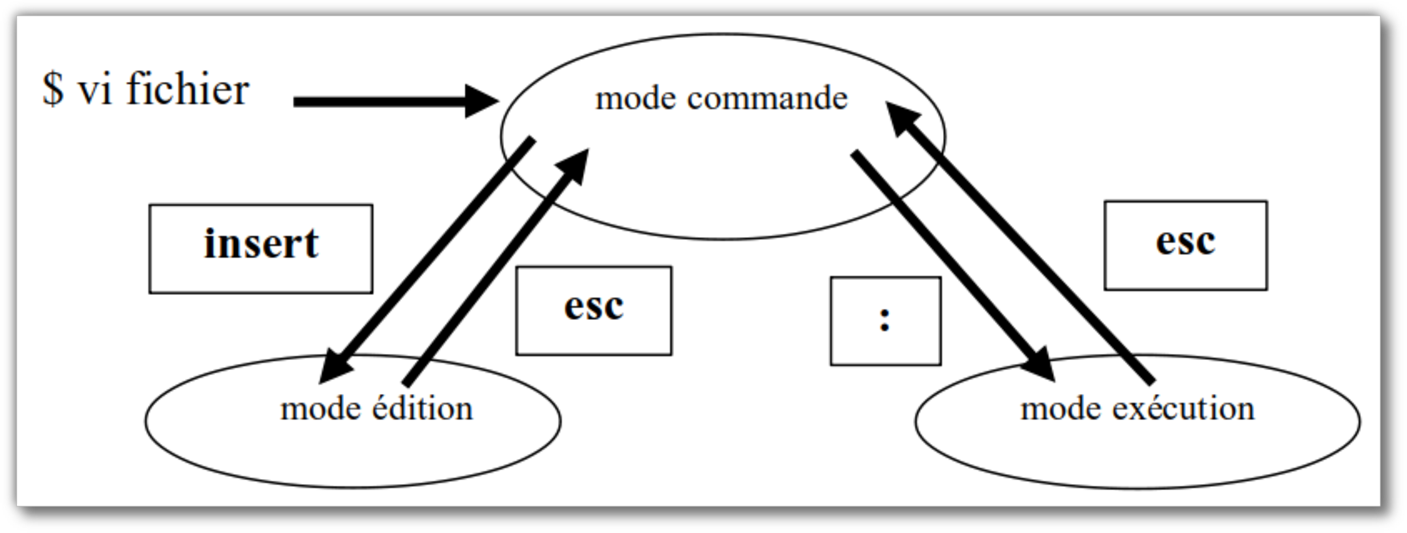
\includegraphics[width=.7\textwidth]{image/vi.pdf}
			\end{center}

		\subsubsection*{Le mode commande}
		%===============================

			C'est le mode dans lequel vous vous trouvez quand vous ouvrez \samp{vi}. 
			Dans ce mode, les touches sur lesquelles vous appuyez
			ne sont pas insérées dans le texte (comme dans nano)
			mais sont considérées comme des commandes.
			C'est le mode qui permet de \textbf{manipuler} le texte.

			Exemples de commandes :
			\begin{itemize}
			\item \kbd{i} : passer en mode édition (cfr. infra);
			\item \kbd{yy} : copier la ligne sous le curseur (comme un \samp{CTRL-C} sous Windows) ; 
			\item \kbd{3yy}	: copier 3 lignes ;
			\item \kbd{dd} : couper la ligne sous le curseur (\kbd{5yy} pour en couper 5) ;
			\item \kbd{dw} : couper le mot sur lequel se trouve le curseur ;
			\item \kbd{p} : coller (ce qui a été précédemment copié ou coupé)
				sous la ligne qui suit le curseur ;
			\item \kbd{u} : annuler la dernière modification. 
				Vous pouvez appuyer plusieurs fois pour annuler les dernières modifications.	
			\end{itemize}

			\subsubsection*{Le mode édition}
			%===============================
		
				C'est le mode dans lequel ce qu'on tape est ajouté au texte,
				comme dans nano.
				On y accède par la touche :
				\begin{itemize}
				\item \kbd{i} (insert) : on insère à l'endroit du curseur ;
				\item \kbd{a} (append) : on insère après le curseur ;
				\item \kbd{o} : on insère dans une nouvelle ligne créée sous le curseur ;
				\end{itemize}

				Dans tous les cas, l'indicateur \texttt{INSERT} 
				apparait alors en bas de l'écran.

			\subsubsection*{Le mode exécution}
			%===============================
			
				On y accède à partir du mode commande en tapant \kbd{:}.
				Ce mode permet d'entrer d'autres types de commandes,
				plus riches que celles du mode commande. 
				Voici les plus utilisées:
				\begin{itemize}
				\item \kbd{:h} pour accéder à l'aide (\kbd{q} pour quitter l'aide) ;
				\item \kbd{:w} pour sauver le fichier ;
				\item \kbd{:w monFichier} pour enregistrer sous \samp{monFichier},
				\item \kbd{:q} pour quitter l'éditeur (sans sauver) ;
				\item \kbd{:x} pour enregistrer et quitter ;
				\item \kbd{:q!} pour quitter sans enregistrer les modifications ;
				\item \kbd{:set nu} pour afficher les numéro de ligne 
					(\kbd{:set nonu} pour les retirer) ;
				\item \kbd{:numéroDeLigne} pour aller directement à cette ligne ;
				\item \kbd{:\%s/old/new/g} 
					pour remplacer toutes les occurrences de la chaine de caractères 
					\samp{old} par la chaine de caractère \samp{new}.
				\end{itemize}
		
\end{document}
			